\documentclass[twocolumn, ]{article}
\usepackage{amsmath}
\usepackage{graphicx}
\usepackage{float}

\usepackage{geometry}
 \geometry{
 a4paper,
 total={170mm,257mm},
 left=5mm,
right=5 mm,
bottom=5 mm,
 top=5mm,
 }
 \usepackage{setspace}
\setstretch{0.1}

\begin{document}

\section*{\small Cheat Sheet for EE464}
\small \begin{equation*}
Form Factor=\frac{V_{rms}}{V_{avg}}
Crest Factor=\frac{V_{peak}}{V_{rms}}
\end{equation*}

\begin{equation*}
Distortion Factor=\frac{I_{1rms}}{I_{rms}}
\end{equation*}
\textit{$\phi$ : phase difference between fundamentals of current and voltage}
\begin{equation*}
Displacement Power Factor=\cos(\phi)
\end{equation*}
\begin{equation*}
True Power Factor=\frac{P}{S}=DPF \frac{I_{1,RMS}}{I_{RMS}}
\end{equation*}
\begin{equation*}
THD=\sqrt{(\frac{I_{rms}}{I_{1rms}})^2-1}
\end{equation*}

Voltages on inductors during on-off times(for ease of waveform drawing) Buck:(Vd-Vo):-Vo;Boost:Vd:-(Vo-Vd); BuckBoost:Vd:-Vo
{Cuk,SEPIC,Flyback:Buck-Boost Topologies;Cuk in-out filter,SEPIC + polarity and energy transfer sharing}

%\begin{figure}[!ht]
%	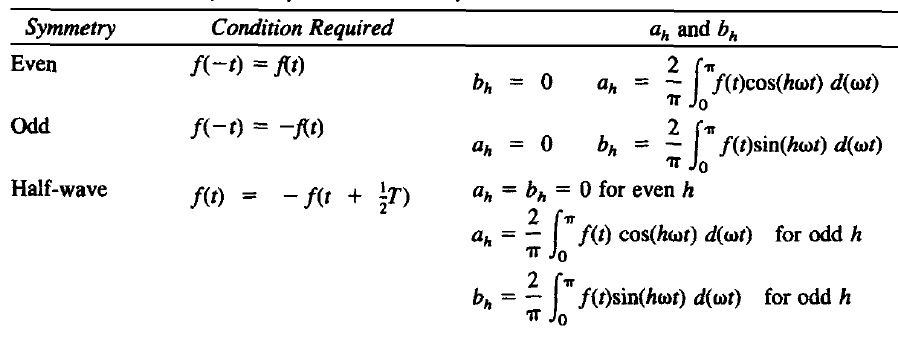
\includegraphics[width=2.5in,height=1in]{fouriert.png}
%	\caption{Fourier Transform Table}
%\end{figure}


\subsubsection*{Converters}

\begin{figure}[!ht]
	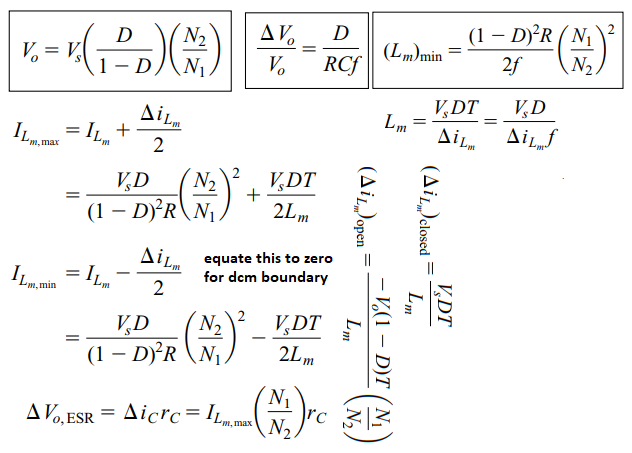
\includegraphics[width=3in,height=1.8in]{flybackformulasfromhart.png}
	\caption{Flyback Formulas}
\end{figure}
\begin{figure}[!ht]
	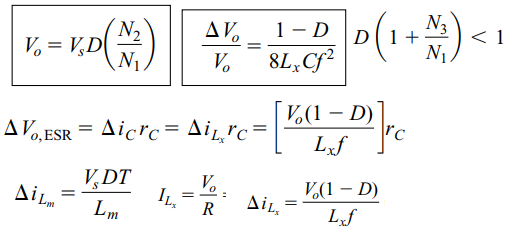
\includegraphics[width=3in,height=1.1in]{forwardsingleswitch.png}
	\caption{Forward (single switched) Converter Formulas}
\end{figure}
\begin{figure}[!ht]
	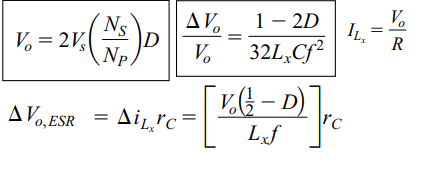
\includegraphics[width=3in,height=0.7in]{pushpull_someformulas.png}
	\caption{Push Pull Formulas}
\end{figure}


%\begin{figure}[!ht]
%	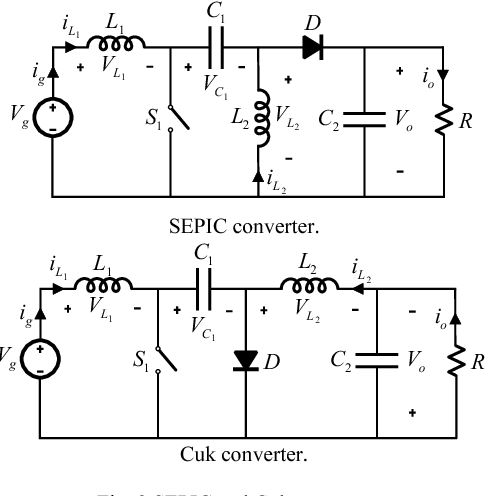
\includegraphics[width=2.5in,height=1.7in]{sepic_and_cuk_schematic.png}
%	\caption{Sepic and Cuk Converter Schematics}
%\end{figure}


\begin{figure}[!ht]
	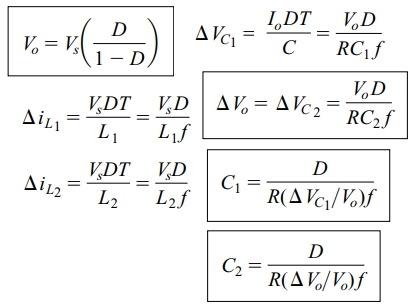
\includegraphics[width=2in,height=1.5in]{sepicformulas.png}
	\caption{Sepic Converter Formulas}
\end{figure}
\begin{figure}[!ht]
	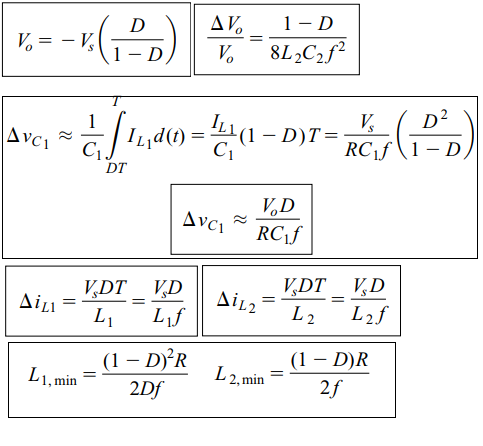
\includegraphics[width=2.2in,height=1.7in]{cukformulas.png}
	\caption{Cuk Converter Formulas}
\end{figure}

  \begin{figure}[!ht]
	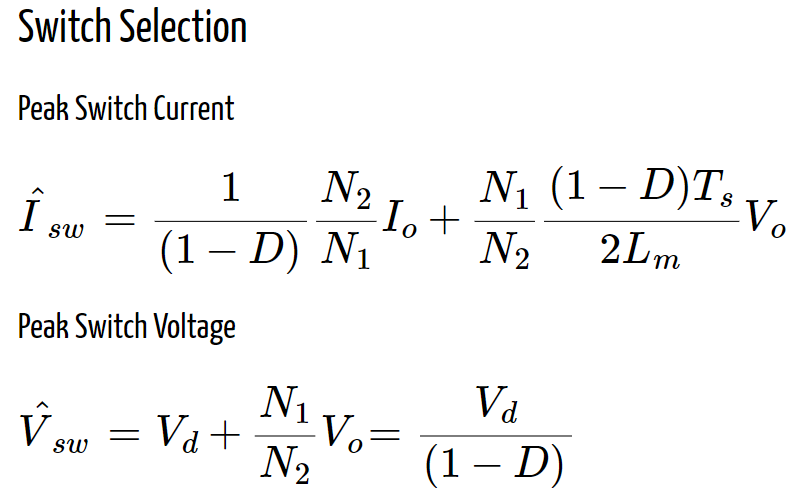
\includegraphics[width=2in,height=1in]{flybak_switch}
	\caption{Flyback switch considerations}
\end{figure}

\begin{figure}[!ht]
	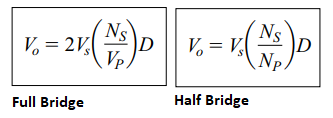
\includegraphics[width=1.6in,height=.6in]{fullandhalfinout.png}
	\caption{Full and Half Bridge Relations}
\end{figure}
%\begin{figure}[!ht]
%	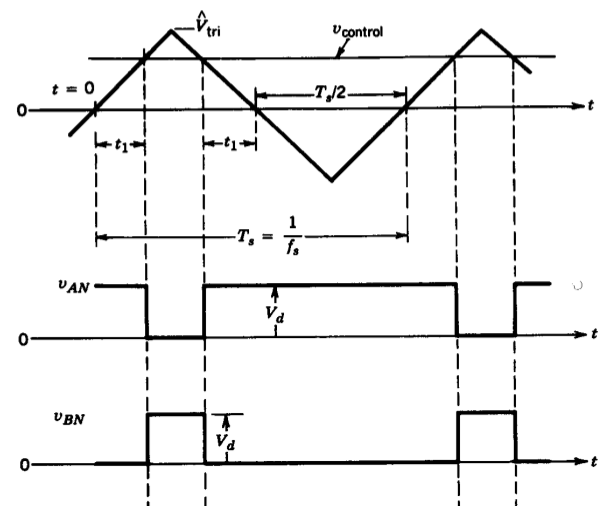
\includegraphics[width=2.5in,height=0.6in]{bipolar1.png}
%	\caption{Bipolar Switching}
%\end{figure}
%\begin{figure}[!ht]
%	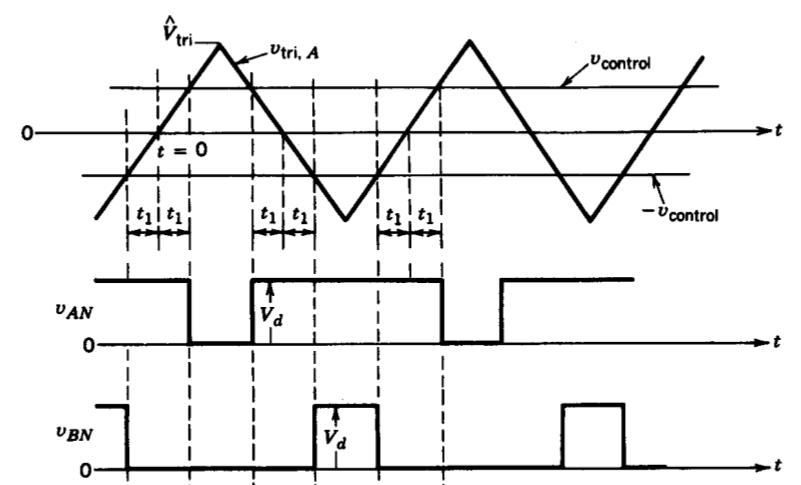
\includegraphics[width=2.5in,height=0.6in]{unipolar1.png}
%	\caption{Unipolar switching}
%\end{figure}

\begin{equation}
Switch Utilization= \frac{Po}{Psw}=\frac{Io.Vo}{q.Vswmax.Iswmax}
\end{equation}

\subsubsection*{Inverters}

$$ m_f=\dfrac{f_s}{f_1}, m_a=\dfrac{V_{control}}{V_{triangle}}$$
$$m_a<1: linear, m_a>1: overmodulation$$

\begin{figure}[!ht]
	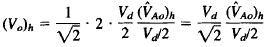
\includegraphics[width=2.3in,height=0.25in]{RmsVoltageofHarmonicsFullBridgeInverter.png}
	\caption{Rms Voltage of Harmonics Full Bridge Inverter}
\end{figure}
%\begin{figure}[!ht]
%	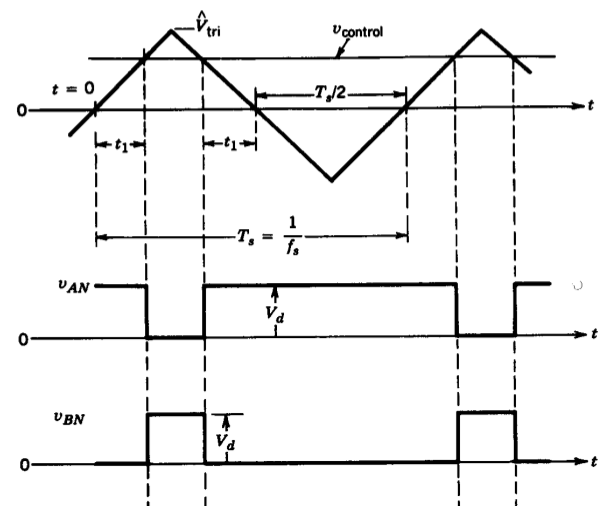
\includegraphics[width=2.5in,height=1in]{bipolar1.png}
%	\caption{Bipolar Switching}
%\end{figure}
%\begin{figure}[!ht]
%	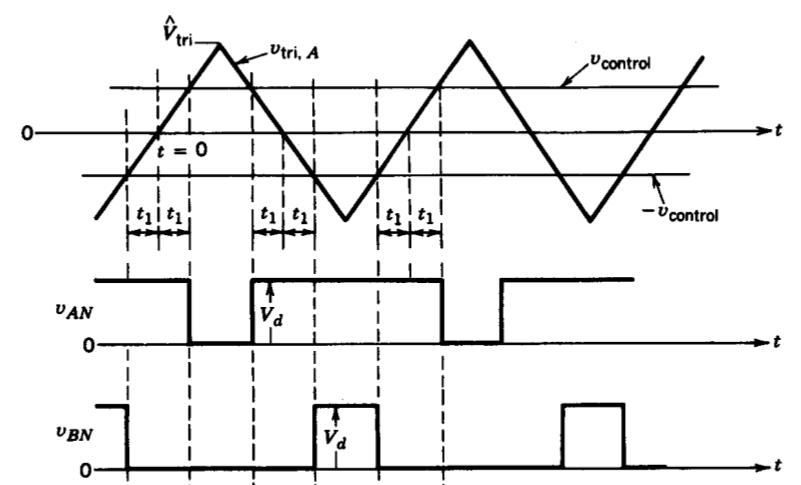
\includegraphics[width=2.5in,height=1in]{unipolar1.png}
%	\caption{Unipolar switching}
%\end{figure}
\subsection*{\small Cuk Converter}
\small
\begin{equation}
Vc1=Vo+Vd
\end{equation}

\begin{equation}
V_{rms}=\frac{2\pi}{\sqrt{2}}.N_{2}.f.B_{max}.A
\end{equation}

Current Source Converter:
\begin{equation}
(V_o = V_d  (\dfrac{N_2}{N_1})(\dfrac{1}{2(1-D)})\\)
\end{equation}

\subsection*{\small Signal Analysis}
 \begin{figure}[!ht]
	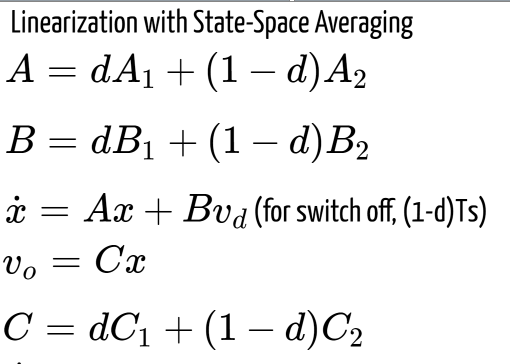
\includegraphics[scale=0.36]{ss1}
\hspace{0.05 cm}
	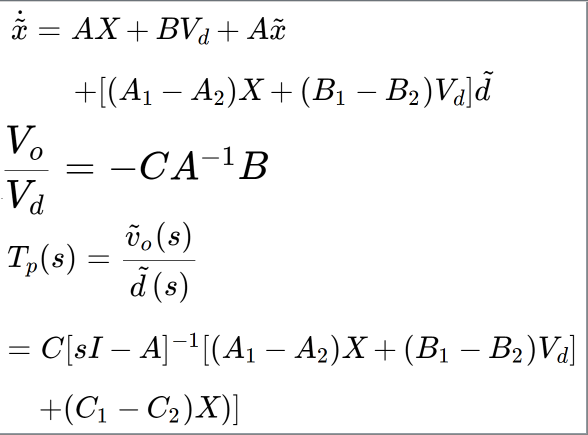
\includegraphics[scale=0.34]{ss2}
\end{figure}
\begin{equation*}
I_{o}=I_{lm}(1-D) 
\hspace{0.2cm}
I_{s}=I_{lm}(D)
\hspace{0.2cm}
At SS: AX+BV_{d}=0
\end{equation*}
For analysis, first derive generalstate space for on and off ccts, then decide which matrices are needed and which are 0. Cct analysis and derive matrices
\begin{table}[H]
\centering
\begin{tabular}{lllll}
    Topology & $V_{sw}$ & $I_{sw}$ & $V_{01,max}$ & q \\
    \hline

    Push Pull & $2V_{d,max}$ & $\sqrt2 \dfrac{I_{o,max}}{n}$ & $\dfrac{4}{\pi \sqrt2} \dfrac{V_{d,max}}{n}$ & 2 \\
    Half B. & $V_{d,max}$ & $\sqrt2 I_{o,max}$ & $\dfrac{4}{\pi \sqrt2} \dfrac{V_{d,max}}{2}$ & 2 \\
    Full B. & $V_{d,max}$ & $\sqrt2 I_{o,max}$ & $\dfrac{4}{\pi \sqrt2} V_{d,max}$ & 4 \\
 \end{tabular}   
  \caption{Swith Utilization doesnt change($1/2\pi$) for n:1 trans. ratio and in linear region scaled by $(m_{a}\pi)/4 $}
  
\end{table}



\end{document}
